%!TEX root = TFG.tex

\chapter{Resultados} \label{chap:result}

Una vez entrenados todos los algoritmos con sus mejores hiperparámetros y con un valor de generalización obtenido de la predicción, tenemos los resultados que se pueden ver en la Fig. \ref{fig:comp_accur}.

\begin{figure}
    \centering
    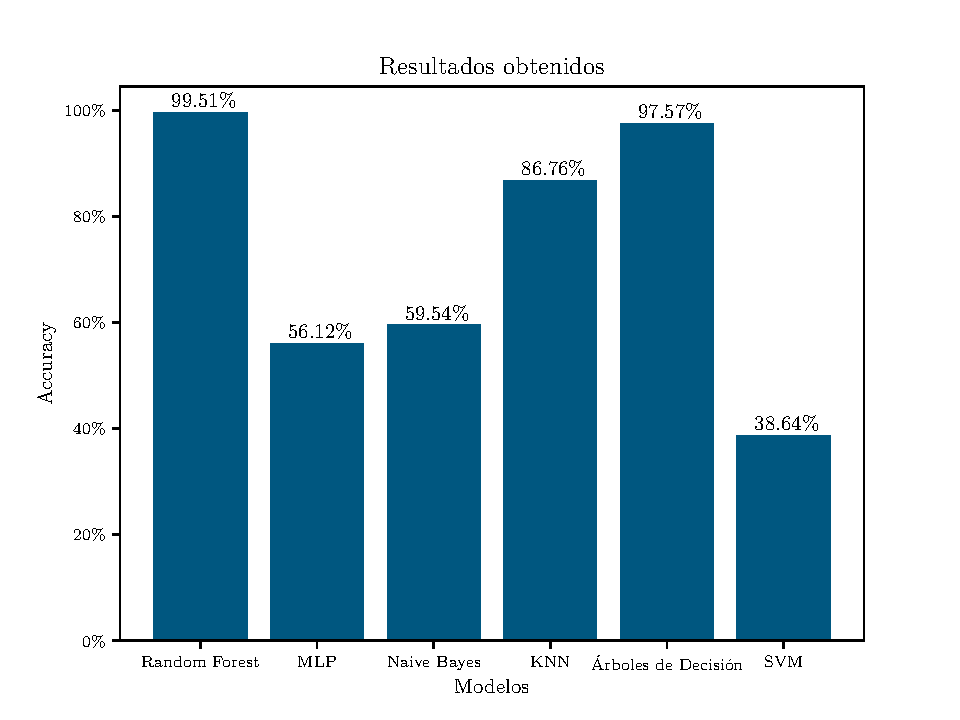
\includegraphics[width=0.4\textwidth]{../Python/plots/parallel/accur_results}
    \caption{Comparativa de resultados entre modelos}
    \label{fig:comp_accur}
\end{figure}

Como se puede ver en ambas muestras los modelos que presentan mejores resultados son los que se basan en árboles de decisión, que son el propio algoritmo de árboles de decisión y random forest. Otra forma de ver estos resultados es mediante las matrices de confusión que nos genera cada algoritmo.

\begin{figure}
    \centering
    \begin{tabular}{ccc}
        \subfloat{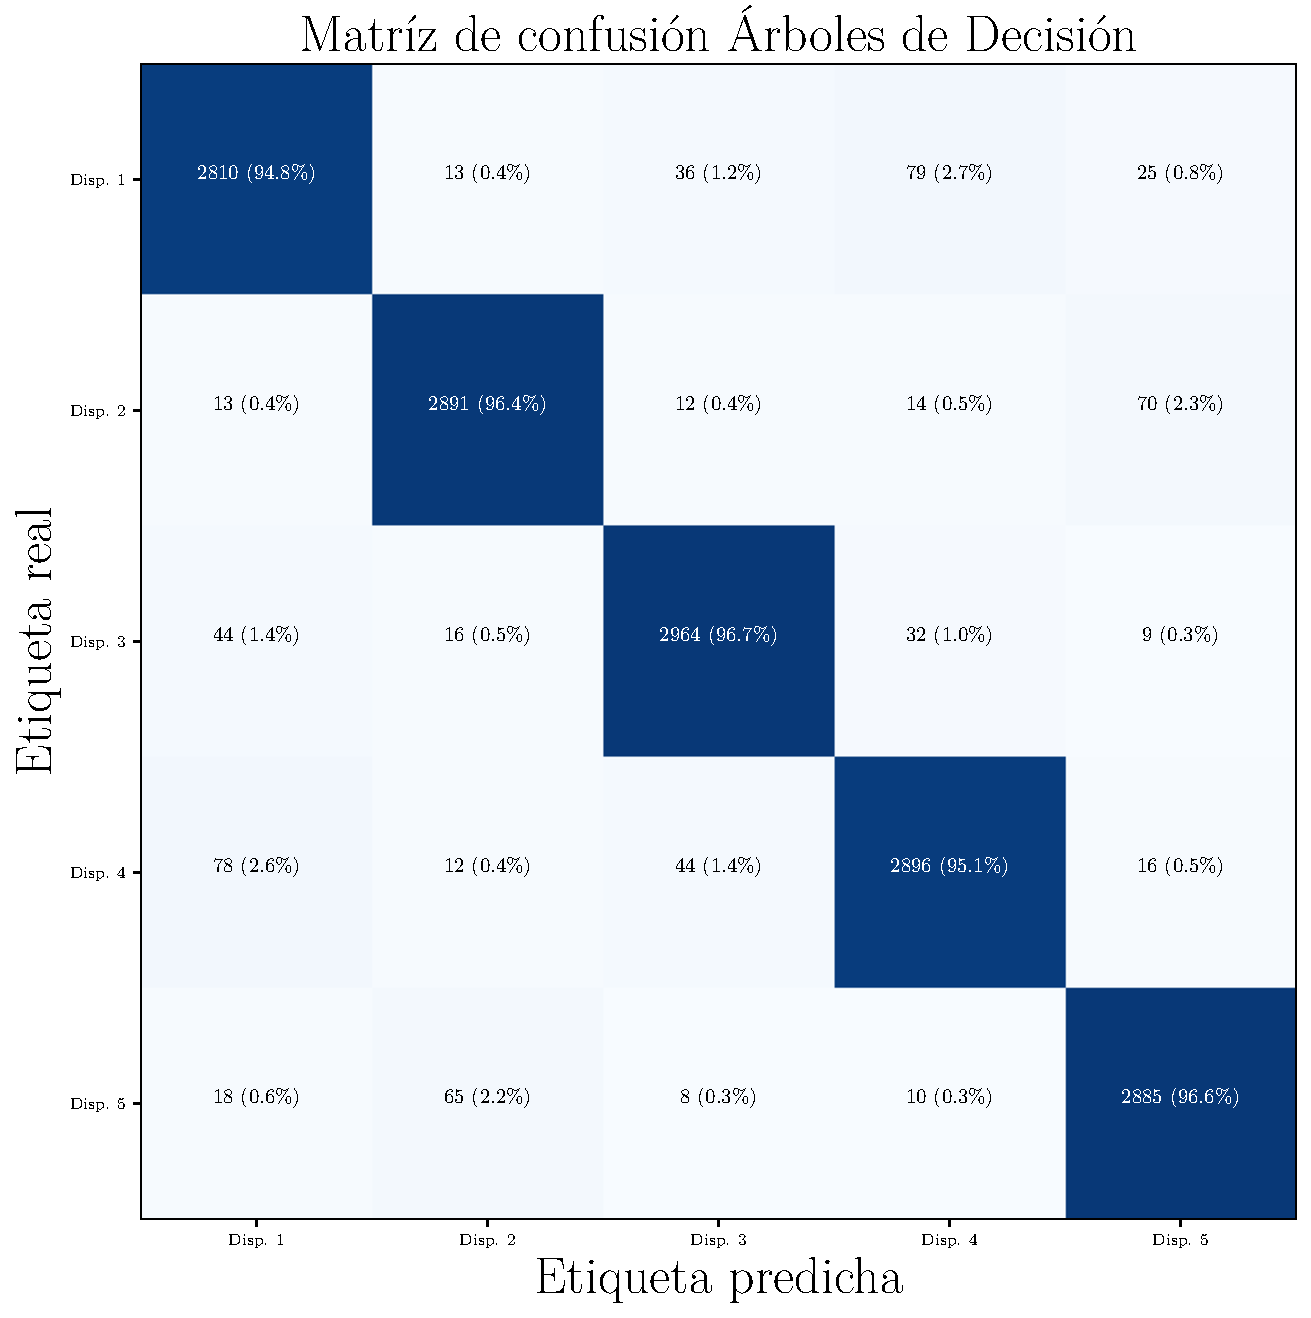
\includegraphics[width=0.4\textwidth]{../Python/plots/parallel/decision_tree_matrix}} & \subfloat{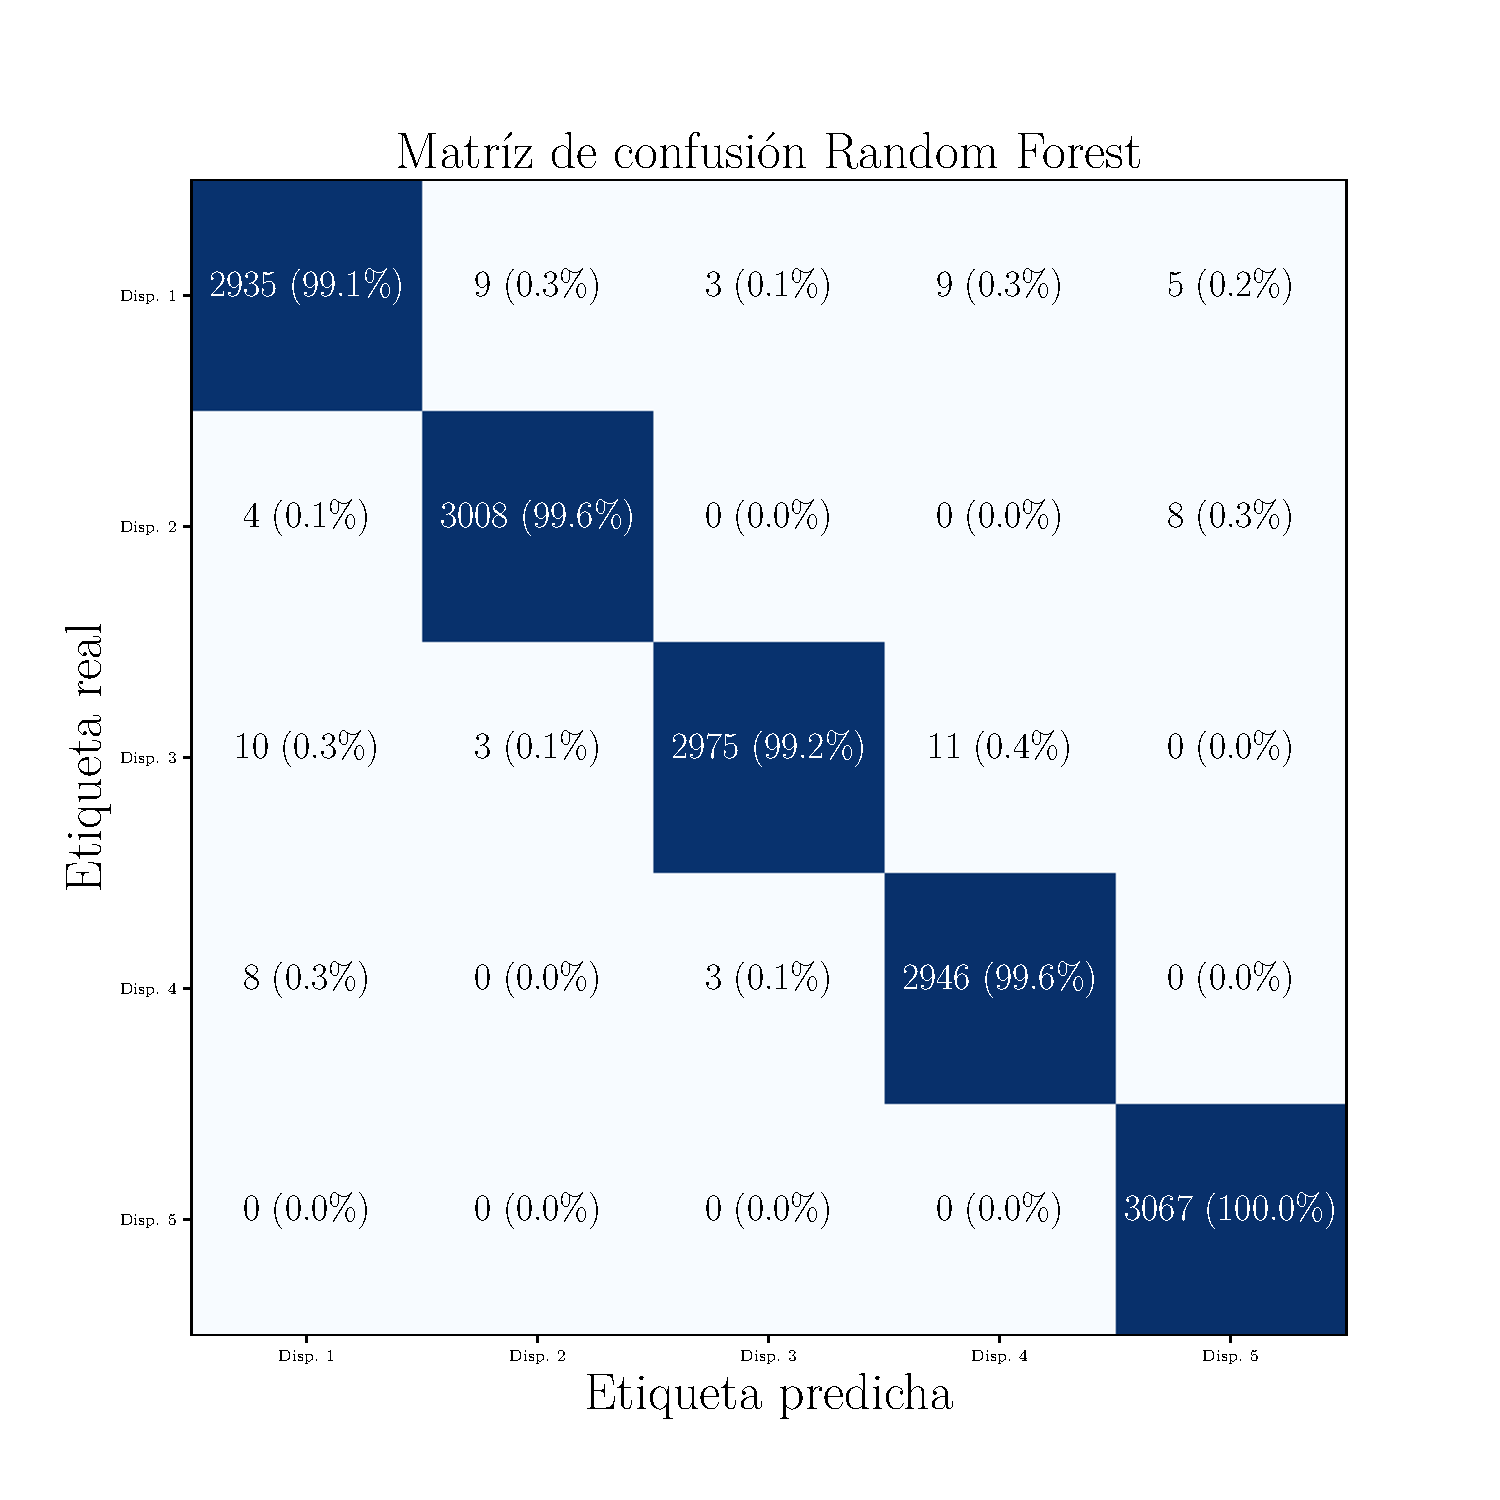
\includegraphics[width=0.4\textwidth]{../Python/plots/parallel/random_forest_matrix}} & \multirow{3}{*}[8em]{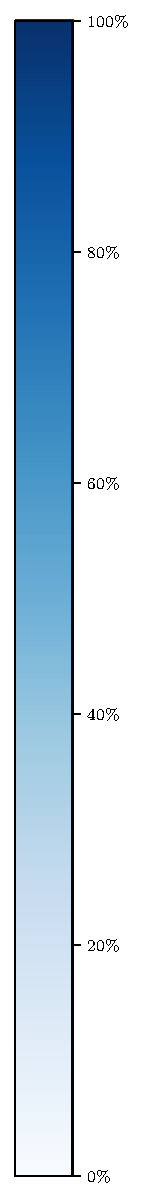
\includegraphics[scale=0.75]{../Python/plots/parallel/colorbar_matrices}} \\
        \subfloat{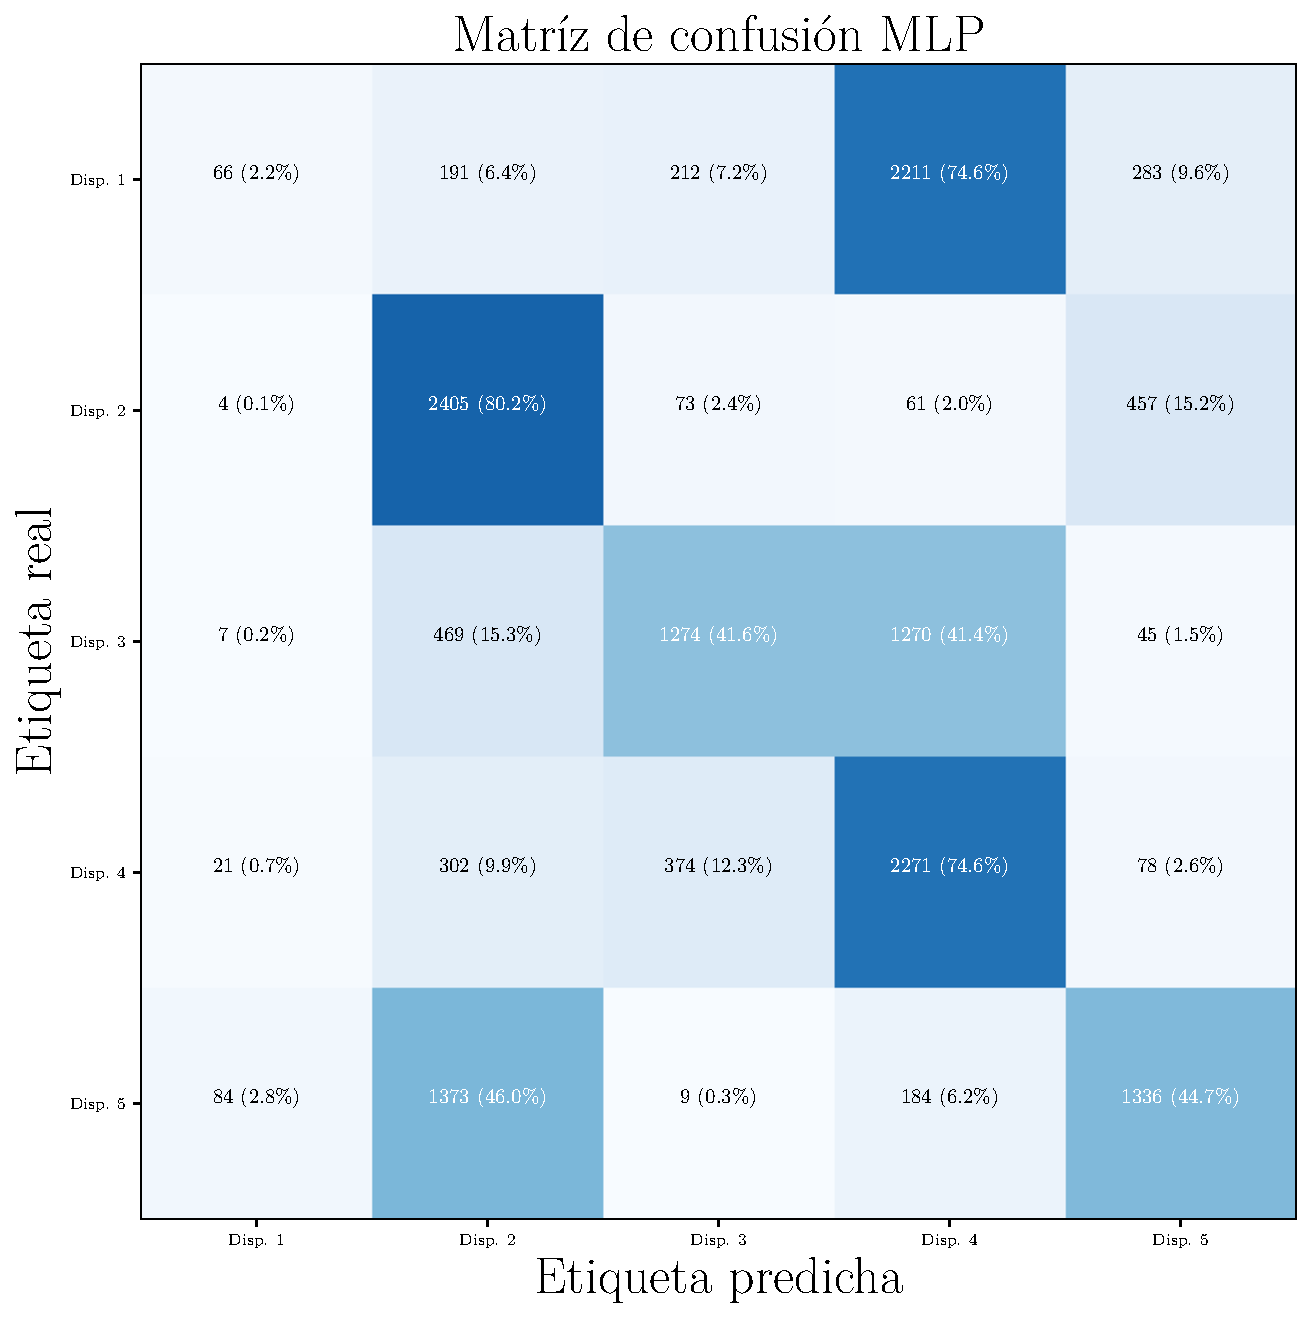
\includegraphics[width=0.4\textwidth]{../Python/plots/parallel/mlp_matrix}} & \subfloat{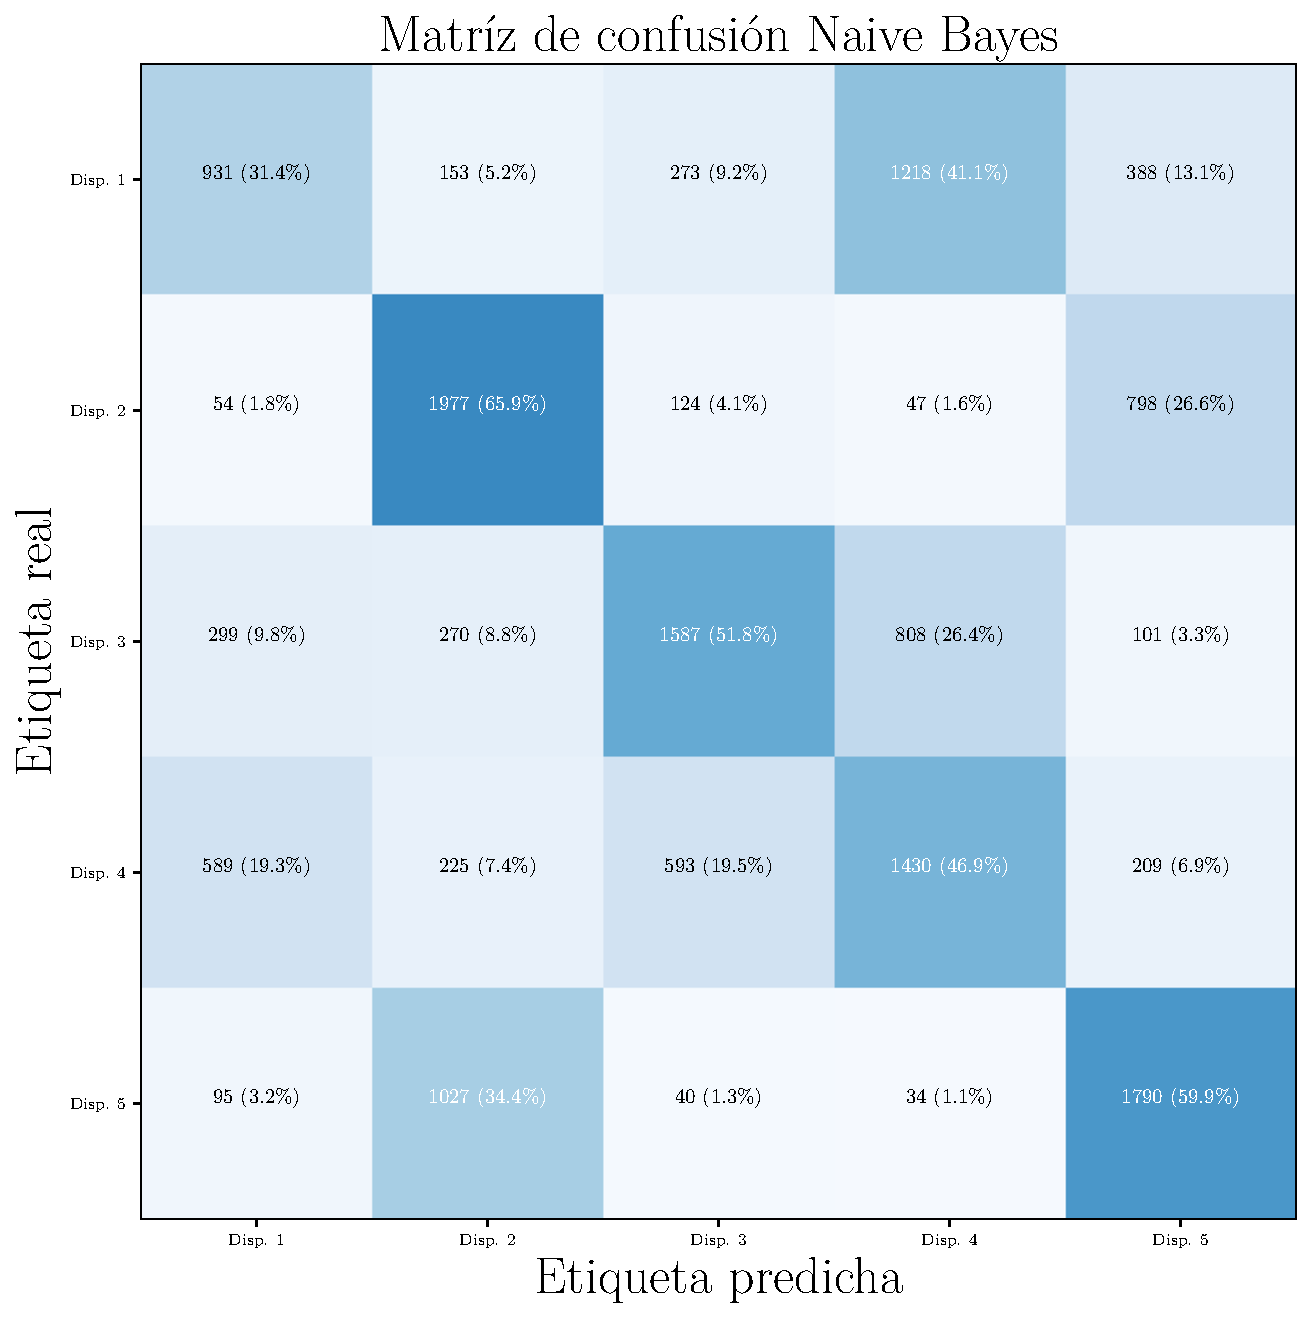
\includegraphics[width=0.4\textwidth]{../Python/plots/parallel/naive_bayes_matrix}} &  \\
        \subfloat{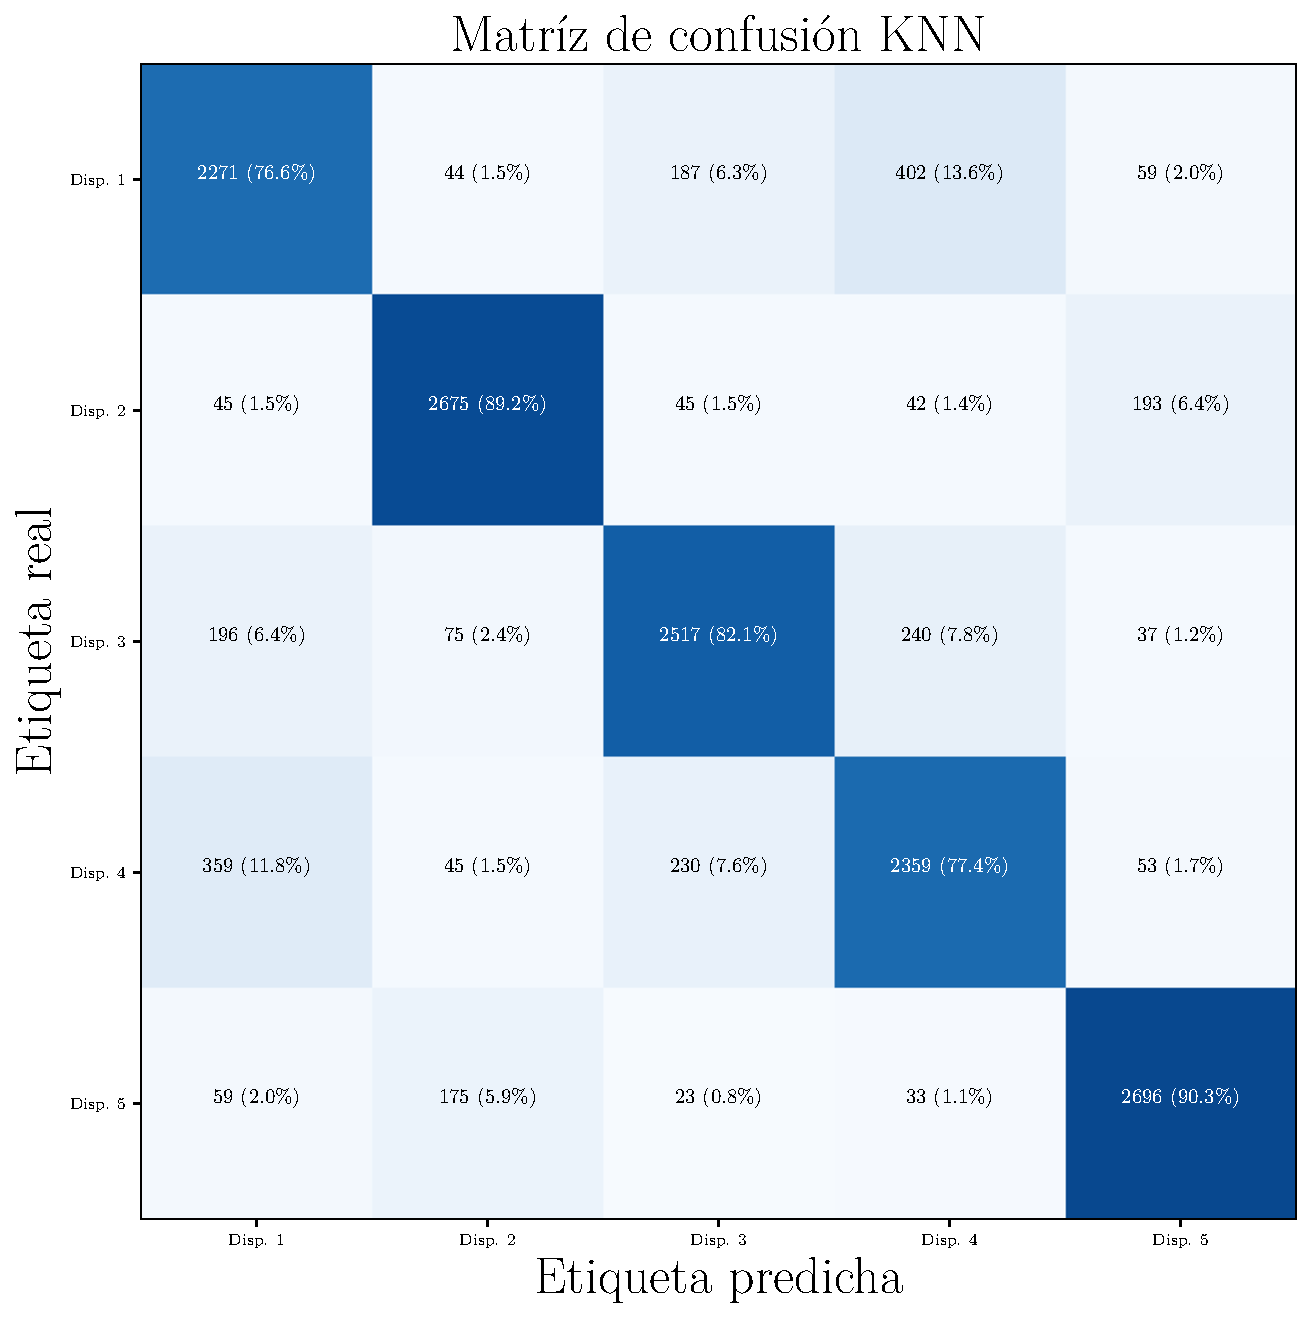
\includegraphics[width=0.4\textwidth]{../Python/plots/parallel/knn_matrix}} & \subfloat{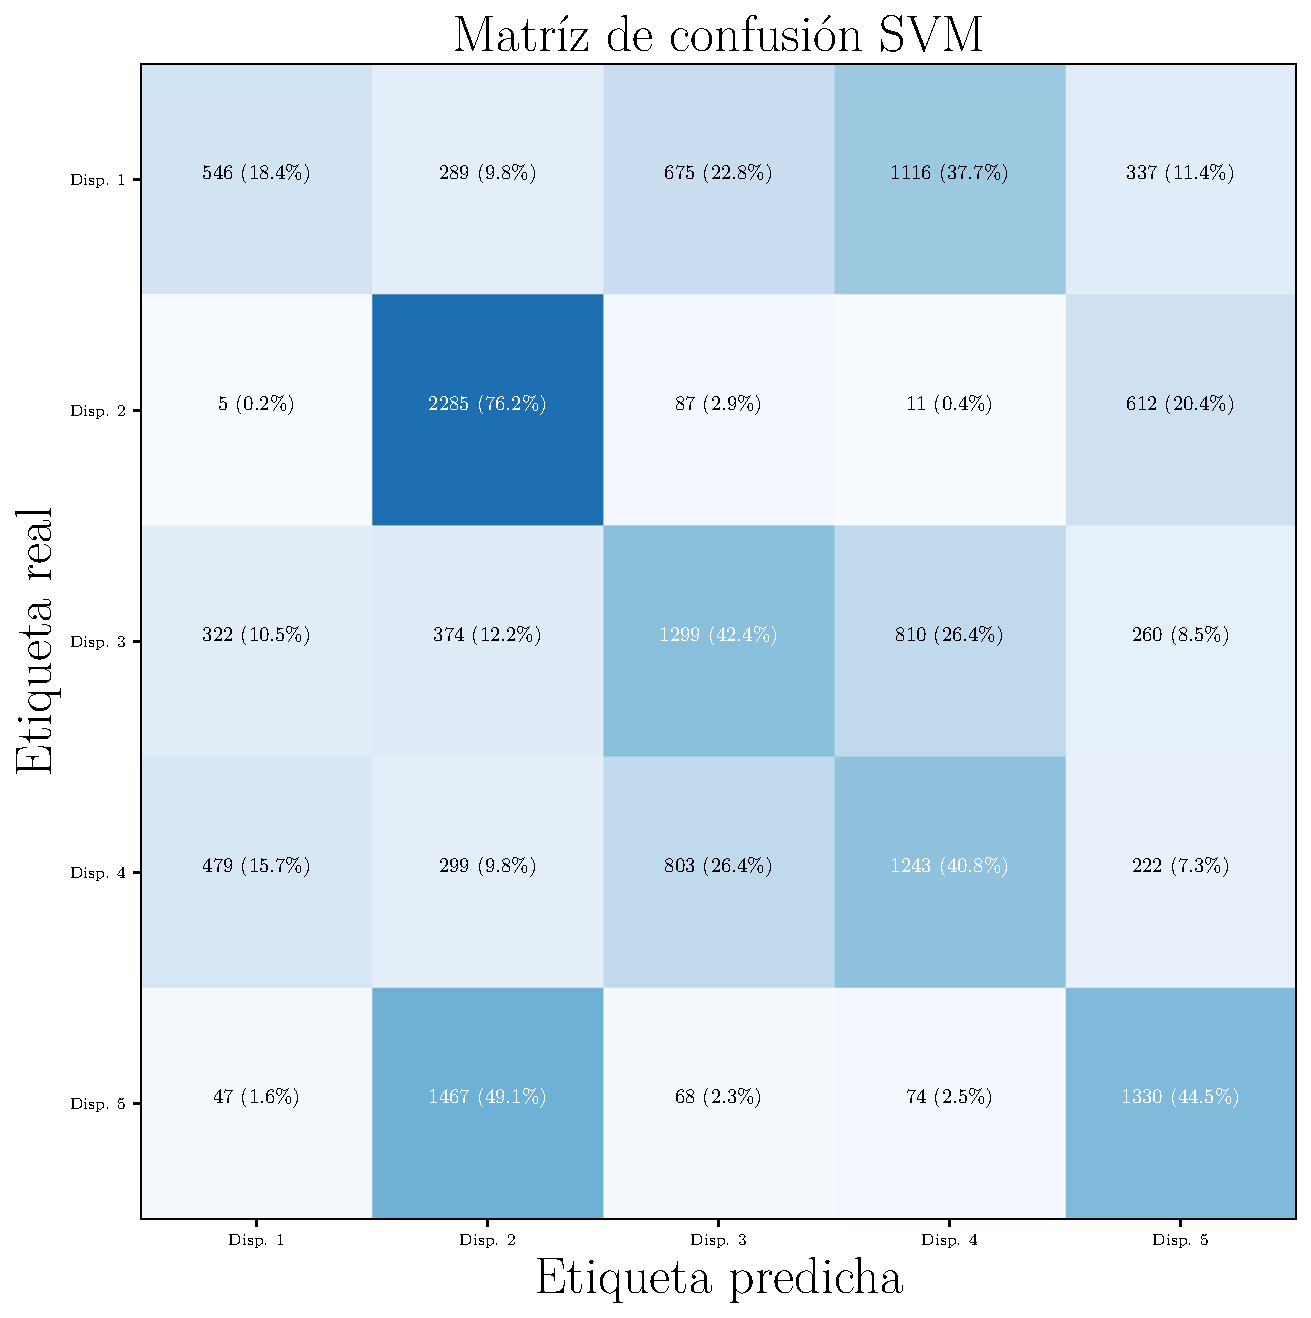
\includegraphics[width=0.4\textwidth]{../Python/plots/parallel/svm_linear_matrix}} & \\
    \end{tabular}
    \caption{Matrices de confusión con datos de la muestra paralela}
    \label{fig:confusion_matrices_parallel}
\end{figure}

Es fácil ver en la Fig. \ref{fig:confusion_matrices_parallel} que los modelos basados en árboles aciertan prácticamente en la totalidad de las ocasiones, en particular, el algoritmo de random forest es el que mejores resultados consigue ($\sim 99.5\%$). Por esta razón se entrenará un modelo de random forest con los hiperparámetros ajustados anteriormente con la totalidad de los datos de entrenamiento. Los resultados obtenidos se pueden ver en la matriz de confusión resultante (Fig. \ref{fig:final_matrix}). Con estos resultados se tiene un valor final de accuracy de 99.44\%.

\begin{figure}[H]
    \centering
    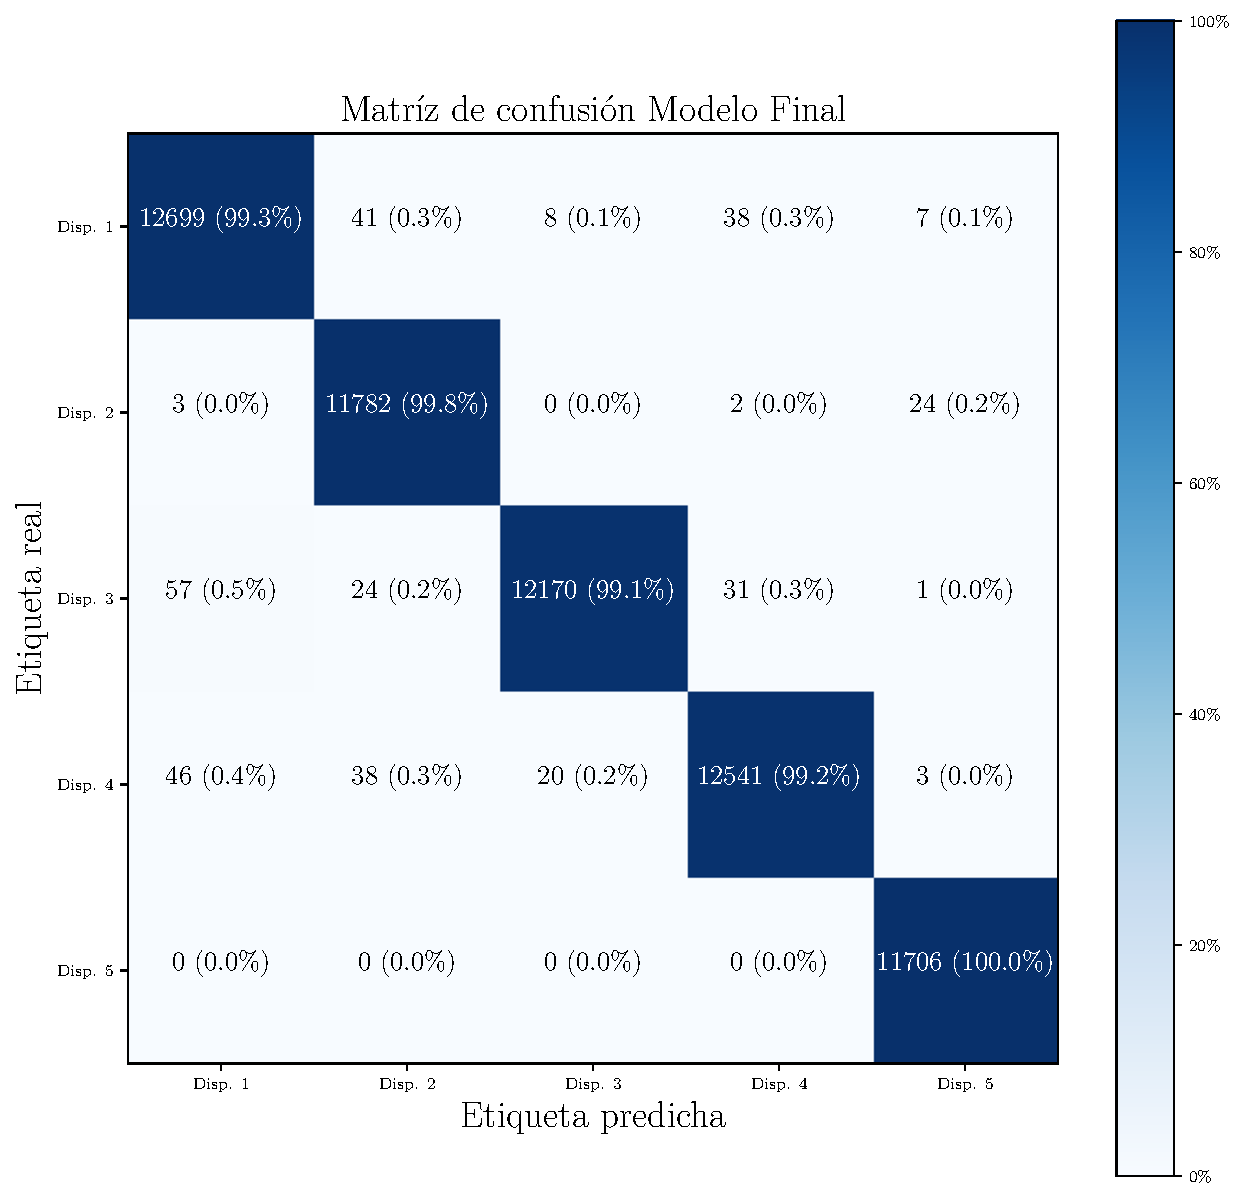
\includegraphics[scale=0.3]{../Python/plots/parallel/final_model_matrix}
    \caption{Matríz de confusión del modelo final}
    \label{fig:final_matrix}
\end{figure}
